\documentclass[paper=a4, fontsize=11pt]{scrartcl}
\usepackage[T1]{fontenc}

\usepackage[english]{babel}															% English language/hyphenation
\usepackage[protrusion=true,expansion=true]{microtype}	
\usepackage{url}
\usepackage{listings}
\usepackage{graphicx}

\usepackage{import}

%%% Custom sectioning
\usepackage{sectsty}
\allsectionsfont{\centering \normalfont\scshape}


%%% Custom headers/footers (fancyhdr package)
\usepackage{fancyhdr}
\pagestyle{fancyplain}
\fancyhead{}											% No page header
\fancyfoot[L]{}											% Empty 
\fancyfoot[C]{}											% Empty
\fancyfoot[R]{\thepage}									% Pagenumbering
\renewcommand{\headrulewidth}{0pt}			% Remove header underlines
\renewcommand{\footrulewidth}{0pt}				% Remove footer underlines
\setlength{\headheight}{13.6pt}

%%% Maketitle metadata
\newcommand{\horrule}[1]{\rule{\linewidth}{#1}} 	% Horizontal rule

\title{
		%\vspace{-1in} 	
		\usefont{OT1}{bch}{b}{n}
		\normalfont \normalsize \textsc{Computer Science Department, University of Crete} \\ [25pt]
		\horrule{0.5pt} \\[0.4cm]
		\huge ICE Editor \\
		\horrule{2pt} \\[0.5cm]
}
\author{\normalfont \normalsize Xenakis Nikolaos\\[-3pt]}
\date{\normalsize Feb - May 2016}

%%% Begin document
\begin{document}
\maketitle
%\href{https://nikosxenakis-website.firebaseapp.com/assets/ICE_Editor/index.html}{ICE Editor}

\section{Abstract}        
	ICE Editor is my bachelor thesis during undergraduate studies in Computer Science department at the University of Crete. This project is a part of a PhD research which main goal is to use efficient means of communication between IOT devices in terms of energy and time using bluetooth technology.

\section{Introduction}
	ICE Editor is a single-page web application which allows an end-user to develop simple applets in IOT devices. This project can be categorized to VPL (Visual Programming Language). The user can easily drop \& drop elements (If, While, For statements etc.) and edit values (variables, arrays, objects etc.). It is an editor which prevents the user to have either compile or runtime (as possible) errors thanks to the strict way of developing code and the runtime checks for valid use of variables.

\section{Description}

	\subsection{Technologies}
		ICE Editor is written using:
		\begin{itemize}
		  \item An HTML file (single-page application)
		  \item Javascript for the main logic of the application
		  \item CSS and LESS technologies for styling
		  \item Jquery framework for faster DOM manipulation
		  \item Bootstrap for the responsive design
		  \item FontAwesome for some basic ui elements like: undo, redo, remove etc.
		  \item  Canvas.js framework for the object rendering
		\end{itemize}

	\subsection{Code Organization}

		\subsubsection{Architecture}
			ICE Editor is designed using Event-driven architecture (EDA) each component has it's own event handlers and performs each action accordingly when triggered.

		\subsubsection{Structure}
			The application uses a middleware layer between Canvas.js and the core in order to create, edit and delete easier and faster programming components. As result, executing: 

			\begin{lstlisting}
				new ForElement (id , elementOffset , father , data);
				/*
				id: unique element id
				elementOffset: position in parent element
				father: reference to parent element
				data: object describing for loop data
				*/
			\end{lstlisting}

			A For element is created. It calls `CreateRectangle()` function that is responsible to call the corresponding functions of Canvas.js that render the shapes.

	\subsection{SideBar}
		The application contains a sidebar a toolbox. The sidebar contains two lists.

		The first is called `Elements` it contains all of the available programming structures (loops, statements and flows) that a user wants to add in his application.
		\begin{figure}[ht!]
		\centering
		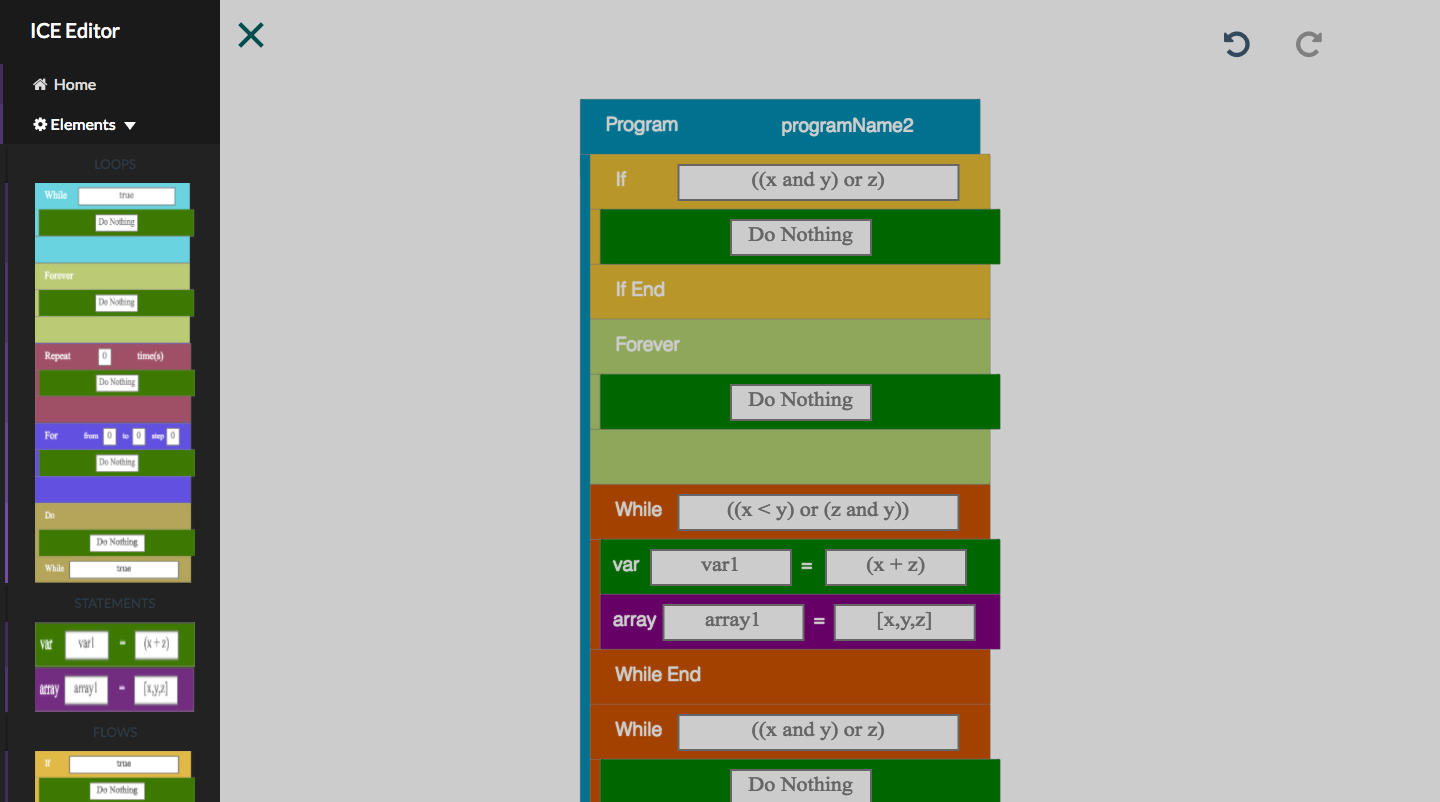
\includegraphics[width=90mm]{images/sideBarElements.jpg}
		\caption{SideBar Elements \label{sideBarElements}}
		\end{figure}


		The second is called `Programs` it contains all of the global variables, functions and programs. In addition, you can add new/delete or see all the functions together.
		\begin{figure}[ht!]
		\centering
		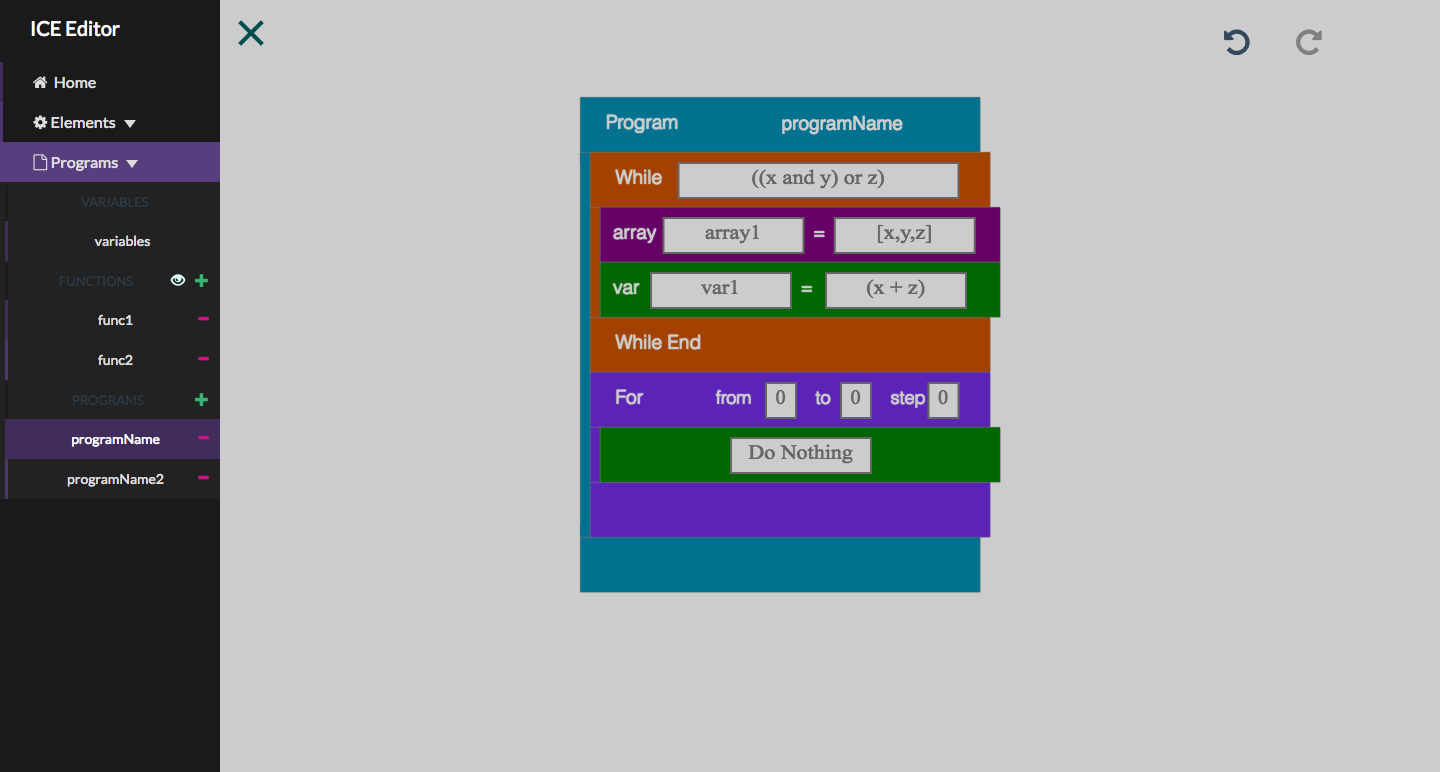
\includegraphics[width=90mm]{images/sideBarPrograms.jpg}
		\caption{SideBar Programs \label{sideBarPrograms}}
		\end{figure}

	\subsection{Edit Elements}
		Users can easily edit an element by tapping in the InputBox of each element. Then a Dialog Menu will pop up.
		\begin{figure}[ht!]
		\centering
		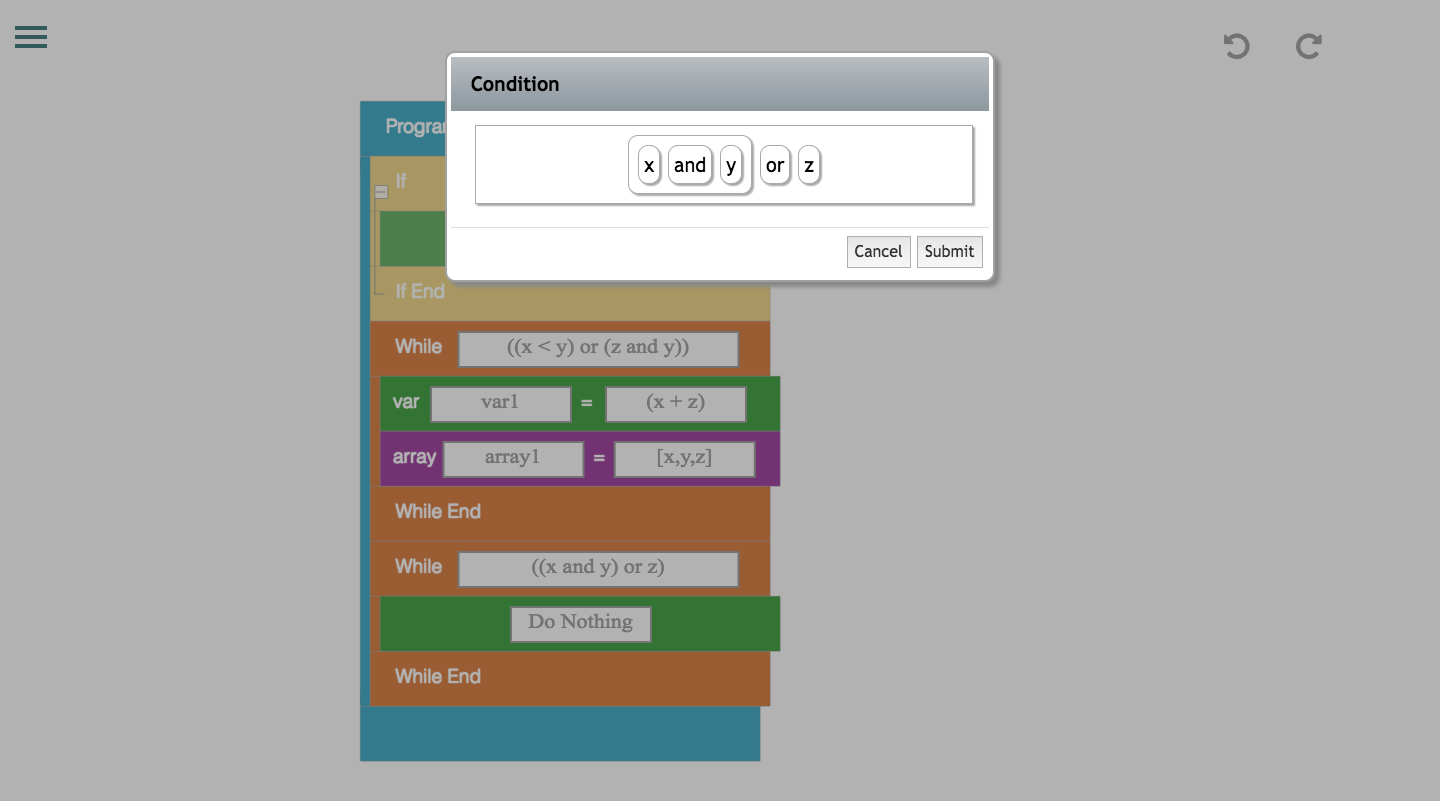
\includegraphics[width=90mm]{images/logicCondition.jpg}
		\caption{Dialog Menu \label{logicCondition}}
		\end{figure}

		There is a variety of those Menus that include Logic, Array, Arithmetic Expressions etc. The most complex Menu is the Logic Expression:
		\begin{figure}[ht!]
		\centering
		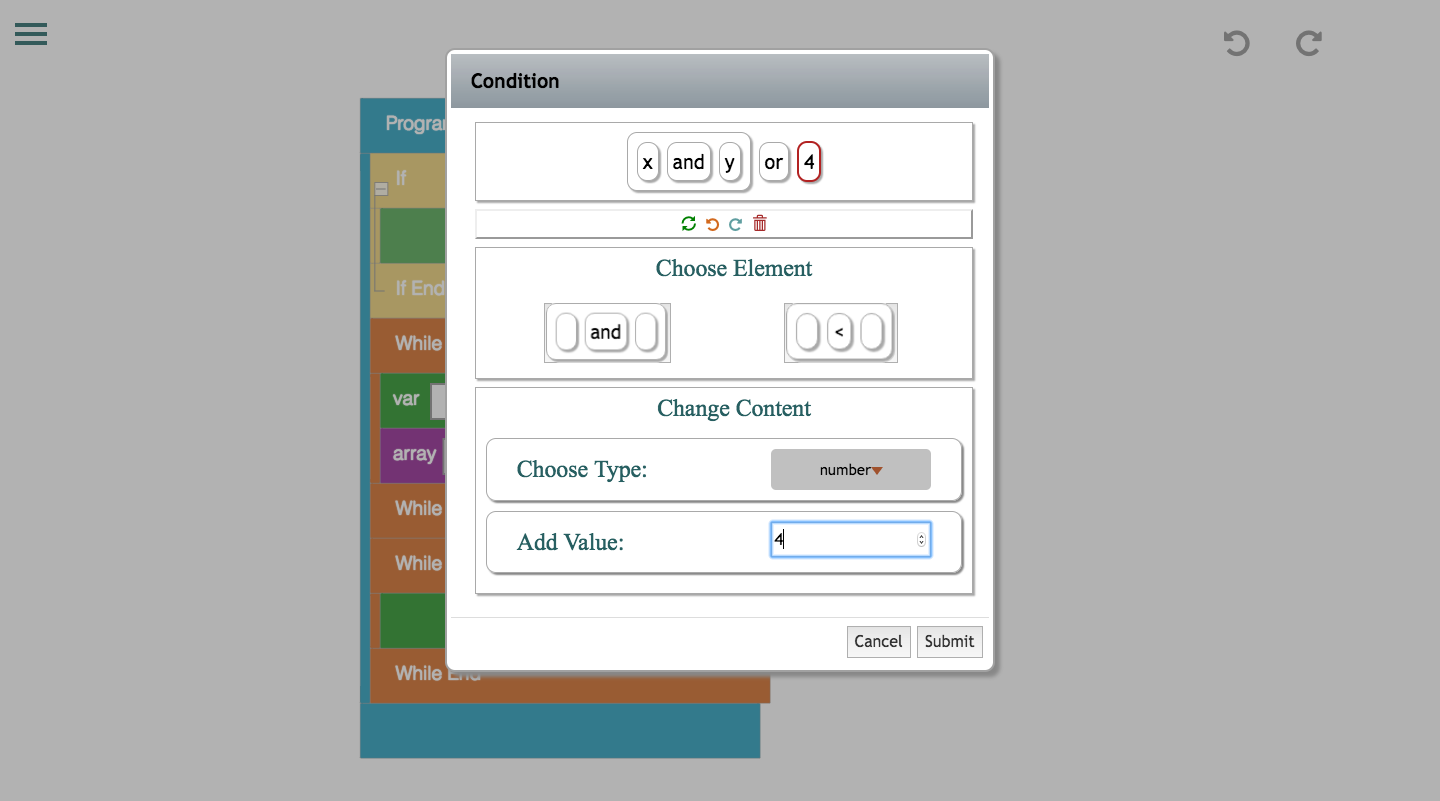
\includegraphics[width=90mm]{images/editCondition.jpg}
		\caption{Logic Expression \label{editCondition}}
		\end{figure}	

		It is plain to see that the user can easily undo/redo refresh and delete it's actions. In addition he can edit an element by clicking on it.

	\subsection{Other Features}

		\subsubsection{Undo/Redo}
			The application supports Undo/Redo feature. The UndoManager uses a stack of functions that are responsible to do the requested action in order to change program's state.

		\subsubsection{See all function}
			It is an option that allows the users to see all of the functions at once in the same workspace.

	\subsection{Input/Output Interaction}
		Users can easily create new programs with two ways. First, by drag \& drop element from the side bar into the canvas and second importing JSON files. For example the following JSON description:

		\begin{lstlisting}
			{
			    id: "myWhile",
			    type: "while",
			    data:{
			        left:{
			            type: InputType.localId,
			            text: "y"
			        },
			        operator:{
			            type: InputType.logicOperator,
			            text: "or"
			        },
			        right:{
			            type: InputType.globalId,
			            text: "z"
			        }
			    },
			    elements:[
			        {
			            id: "myAssign",
			            type: "assign",
			            data:{
			                varName: "myGVar",
			                varType: "globalId",
			                arithmeticExpression:{
			                    type: InputType.number,
			                    text: "3"
			                }
			            }
			        },
			    ]
			}
		\end{lstlisting}
		Creates this code that is rendered in the Canvas as an ICE Editor's element.:
		\begin{lstlisting}
			while(y or z)
				myGVar = 3;
		\end{lstlisting}
		
		Vice verca the user can export a created application into a JSON file in order to save the project.

%%% End document
\end{document}